We discussed the cluster algorithm for the 2d Ising model in class. We saw that the
partition function could be written as
%
\begin{equation}
    Z = \sum_{\{\sigma\}} \prod_{\langle i j \rangle} \sum_{n_{ij}=0}^1
    \bigl((1 - p) \delta_{n_{ij},0} + p \delta_{\sigma_i,\sigma_j} \delta_{n_{ij},1}\bigr),
\end{equation}
%
in the Swendsen--Wang algorithm,
where \(\langle i j \rangle\) refers to all nearest neighbour pairs of atoms.
In this problem, you should start from this code and add measurements to measure the
correlation length near the critical value of \(J\), or \(P=1 - \exp(-2J)\).

In this problem, you should measure the spatial correlation between spins. The simplest
correlator is
%
\begin{equation}
    \expval{ \sigma(x_1, y_1) \sigma(x_2, y_2) }.
\end{equation}
%
But the statistical errors are much smaller if on each configuration of an \(N \times N\)
lattice you calculate
%
\begin{equation}
    \Sigma_x(x) = \frac{ 1 }{ N } \sum_y \sigma(x, y),
\end{equation}
%
and
%
\begin{equation}
    \Sigma_y(y) = \frac{ 1 }{ N } \sum_x \sigma(x, y),
\end{equation}
%
and then calculate
%
\begin{equation}\label{eq:Sigmaz}
    \Sigma(z) = \frac{ 1 }{ 2N } \biggl( \sum_x \Sigma_x(x) \Sigma_x(x+z)
    + \sum_y \Sigma_y(y) \Sigma_y(y+z) \biggr).
\end{equation}
%
On a periodic lattice, the ensemble average \(\expval{\Sigma(z)}\) is only a
function of \(\abs{z}\). Above \(T_c\),
where there is no spontaneous magnetization, \(\expval{\Sigma(z)}\) has the form
%
\begin{equation}\label{eq:Sigmazbar}
    \expval{\Sigma(z)} = a \bigl(\exp(-z / b) + \exp(-(N - z) / b)\bigr).
\end{equation}

\subsection{Measuring this observable}

Measure the correlation in \(\eqref{eq:Sigmaz}\). Even
though the cluster algorithm produces decorrelated configurations quite rapidly, you should
still do some number of spin-flip updates between each measurement. Ten updates is a
reasonable choice.

When you measure \(\eqref{eq:Sigmaz}\) on a configuration, you will end up with \(N\)
values, one for each value of \(z\). For each value of \(z\), you can also determine the
error on the average value using the statistical methods of Problem Set 3.

\Question{} Measure \(\eqref{eq:Sigmaz}\) on systems with values for \(J\) of \(0.435\),
\(0.430\), \(0.425\). (Note that the critical value is \(J_c = 0.4406868\) and higher
temperatures correspond to lower values of \(J\), since we wrote \(J = \bar{J} / k_B T\).

\Answer{}
In the following text, we will set all of the initial spins up and let it evolve.
There are \(5000\) steps in each simulation, while we only take thermalized steps
(from \(3000\) to \(5000\)) into account.
For a fixed lattice size (\(32\) for example) and a fixed \(J\),
we calculate \(\Sigma(z)\) for each configuration and average them to obtain the
ensemble average \(\expval{\Sigma(z)}\).
We also measure the standard deviation of all configurations at each \(z\),
and use them as the \(y\)-error for our data.
The results are plotted in Figure~\ref{fig:cor_N=32_bin=1},
where the scatters are the raw data for \(\expval{\Sigma(z)}\) at each \(z\)
for each \(J\).

\begin{figure}
    \centering
    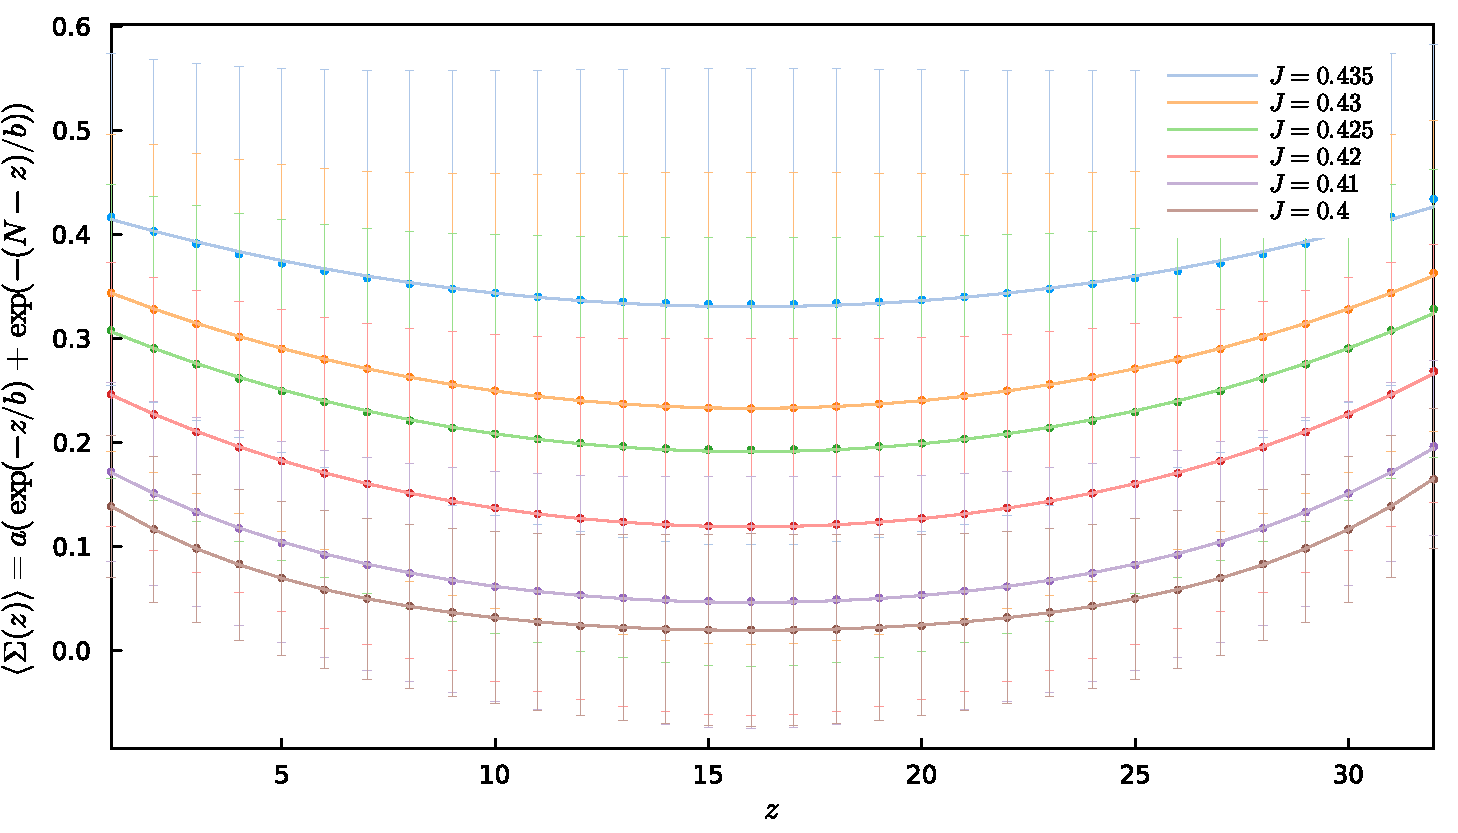
\includegraphics[width=0.9\textwidth]{correlation_N=32_b=1}
    \caption{Ensemble averages \(\expval{\Sigma(z)}\) as a function of \(z\) for different
        \(J\) (above \(T_c\)). The system is a \(32 \times 32\) square lattice
        with all spin up as its initial value.}
    \label{fig:cor_N=32_bin=1}
\end{figure}

\begin{figure}[H]
    \centering
    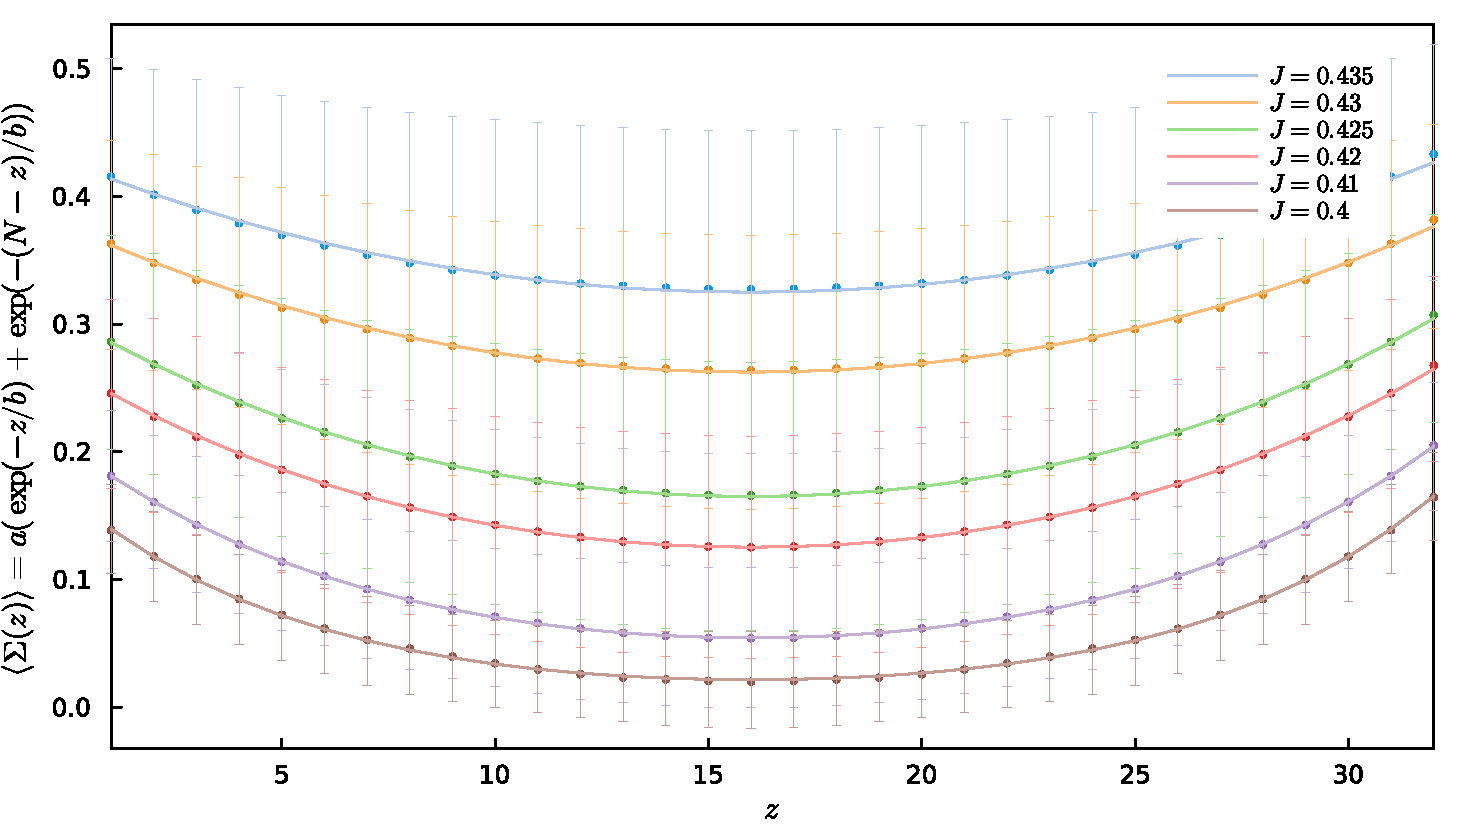
\includegraphics[width=0.9\textwidth]{correlation_N=32_b=20}
    \caption{Ensemble averages \(\expval{\Sigma(z)}\) as a function of \(z\) for different
        \(J\) (above \(T_c\)). The system is a \(32 \times 32\) square lattice
        with all spin up as its initial value.
        We group \(20\) steps into one group, leaving \(3000 / 20 = 150\) groups.}
    \label{fig:cor_N=32_bin=20}
\end{figure}

As we can see, as temperature increases (\(J\) decreases), all the values of
\(\expval{\Sigma(z)}\) tend to decrease.
This is expected since, above the critical temperature, the correlation length
decreases as temperature increases.
And the larger \(z\) is, the lower the correlation is between any two sites.
Therefore, we can observe a minimum of \(\expval{\Sigma(z)}\) around \(N / 2\).
We can also observe that the error bars are relatively large, especially for
larger \(J\)s (lower temperatures).
We learn from Figure~\ref{fig:mag_J=0.41} and~\ref{fig:mag_J=0.435_cluster}
that, when the temperature is closer to \(T_c\), there will be more fluctuations.
In other words, larger standard deviation.
Also, we are plotting the standard deviation for each configuration,
not the standard deviation of the means (by grouping several configurations together).
We can group all configurations into smaller samples, e.g., each of them
is of size \(20\), as long as the group size is larger but not too far away from
the integrated autocorrelation time. With this method, the error bars will shrink
a little, as shown in Figure~\ref{fig:cor_N=32_bin=20}.
However, they are still a bit large. To further shrink the error bars,
we can use the jackknife resampling technique.
The jackknife standard deviation is \(\sqrt{1 / N}\) that of the original dataset,
as shown in Figure~\ref{fig:cor_N=32_bin=20_jack}.

\begin{figure}
    \centering
    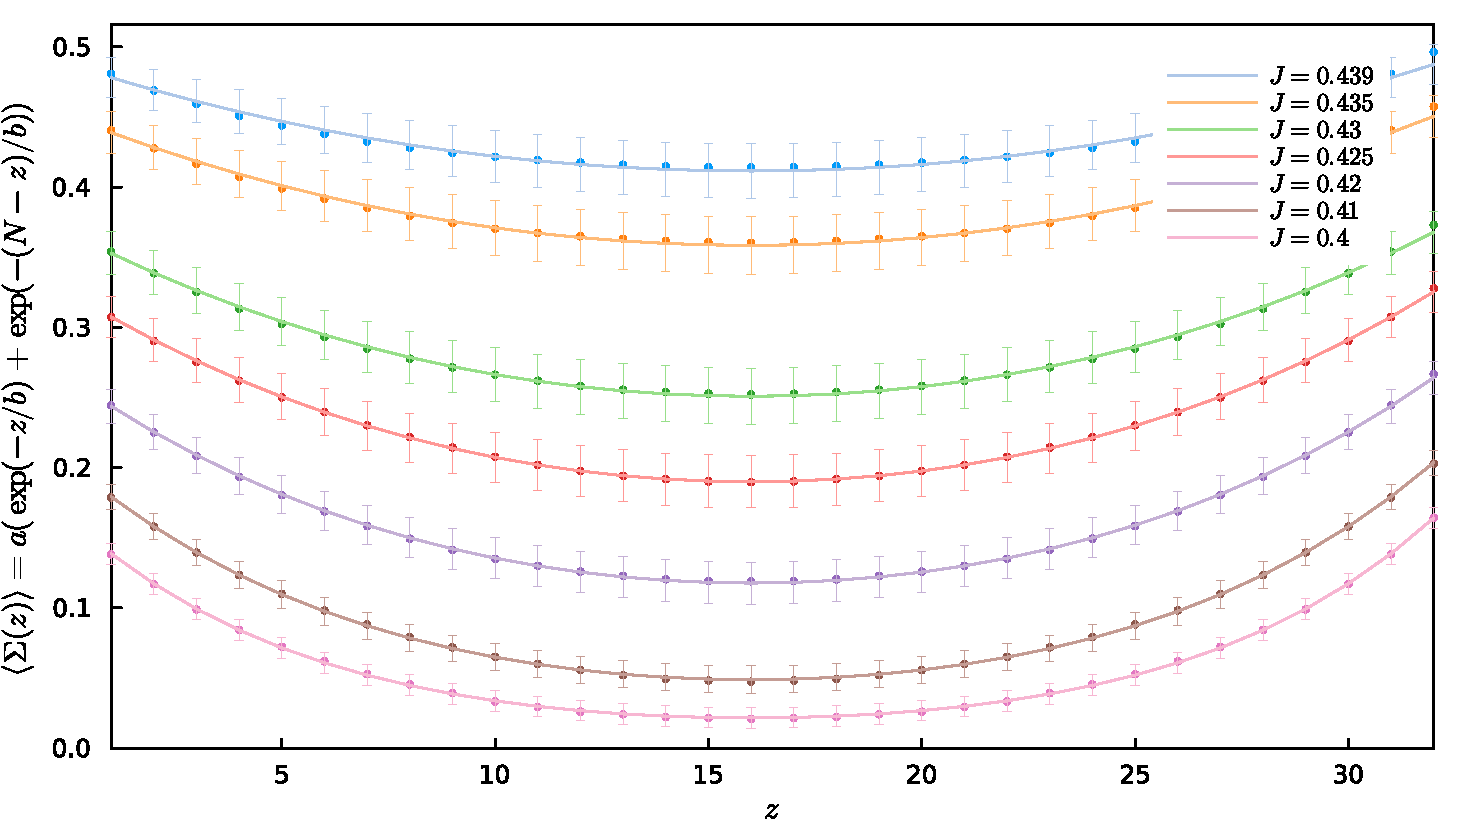
\includegraphics[width=0.9\textwidth]{correlation_N=32_b=20_jack}
    \caption{Ensemble averages \(\expval{\Sigma(z)}\) as a function of \(z\) for different
        \(J\) (above \(T_c\)). The system is a \(32 \times 32\) square lattice
        with all spin up as its initial value.
        We group \(20\) steps into one group, leaving \(3000 / 20 = 150\) groups.
        The data and standard deviations are calculated using the jackknife method.}
    \label{fig:cor_N=32_bin=20_jack}
\end{figure}

\subsection{Determining the correlation length}

In \(\eqref{eq:Sigmazbar}\), \(b\) is the correlation length, which should grow as
\(J \rightarrow J_c\).

\Question{} You can fit your data to the form of \(\eqref{eq:Sigmazbar}\) to find \(b\)
using the curve fit function \code{curve_fit} from
\href{https://github.com/JuliaNLSolvers/LsqFit.jl}{\code{LsqFit.jl}}.

You should include the statistical error on each correlator point in your inputs to
\code{curve_fit}.
You don't need to calculate the error on the returned value of the correlation length,
\(b\), but this can be done with jackknife methods.

Report on your determination of \(b\) for each of the \(J\) values you
simulated. Do you find the expected change in \(b\) as \(J \rightarrow J_c\)?

\Answer{}
We fit Equation~\eqref{eq:Sigmazbar} using \code{LsqFit.curve_fit}.
The fitted function as a function of \(z\) is plotted in Figure~\ref{fig:cor_N=32_bin=1}
to Figure~\ref{fig:cor_N=32_bin=20_jack} as solid lines.
We can see they match our raw values of \(\expval{\Sigma(z)}\) pretty well.

To better observe the relation between fitted values of \(b\) and parameter \(J\),
we plot them in Figure~\ref{fig:b_J_n=32}.
Apparently, as temperature increases (\(J\) decreases), the correlation length \(b\)
decreases. The closer to the critical temperature \(T_c\), the larger the correlation
length will be. Because at \(T_c\), the correlation length is infinite.
At \(J = 0.435\), \(b \approx 21.0326\), which is already close to the size of the lattice.
It explains the relatively significant correlation in Figure~\ref{fig:cor_N=32_bin=20_jack}.

\begin{figure}[hb]
    \centering
    \includegraphics[width=0.9\textwidth]{b(J)_N=32}
    \caption{Fitted parameter \(b\) as a function of \(J\) for a \(32 \times 32\)
        square lattice.}
    \label{fig:b_J_n=32}
\end{figure}
